
\section{Durchführung}
\label{sec:Durchführung}
\renewcommand{\labelenumi}{\alph{enumi})}
\begin{enumerate}


  \begin{figure}[H]
    \centering
    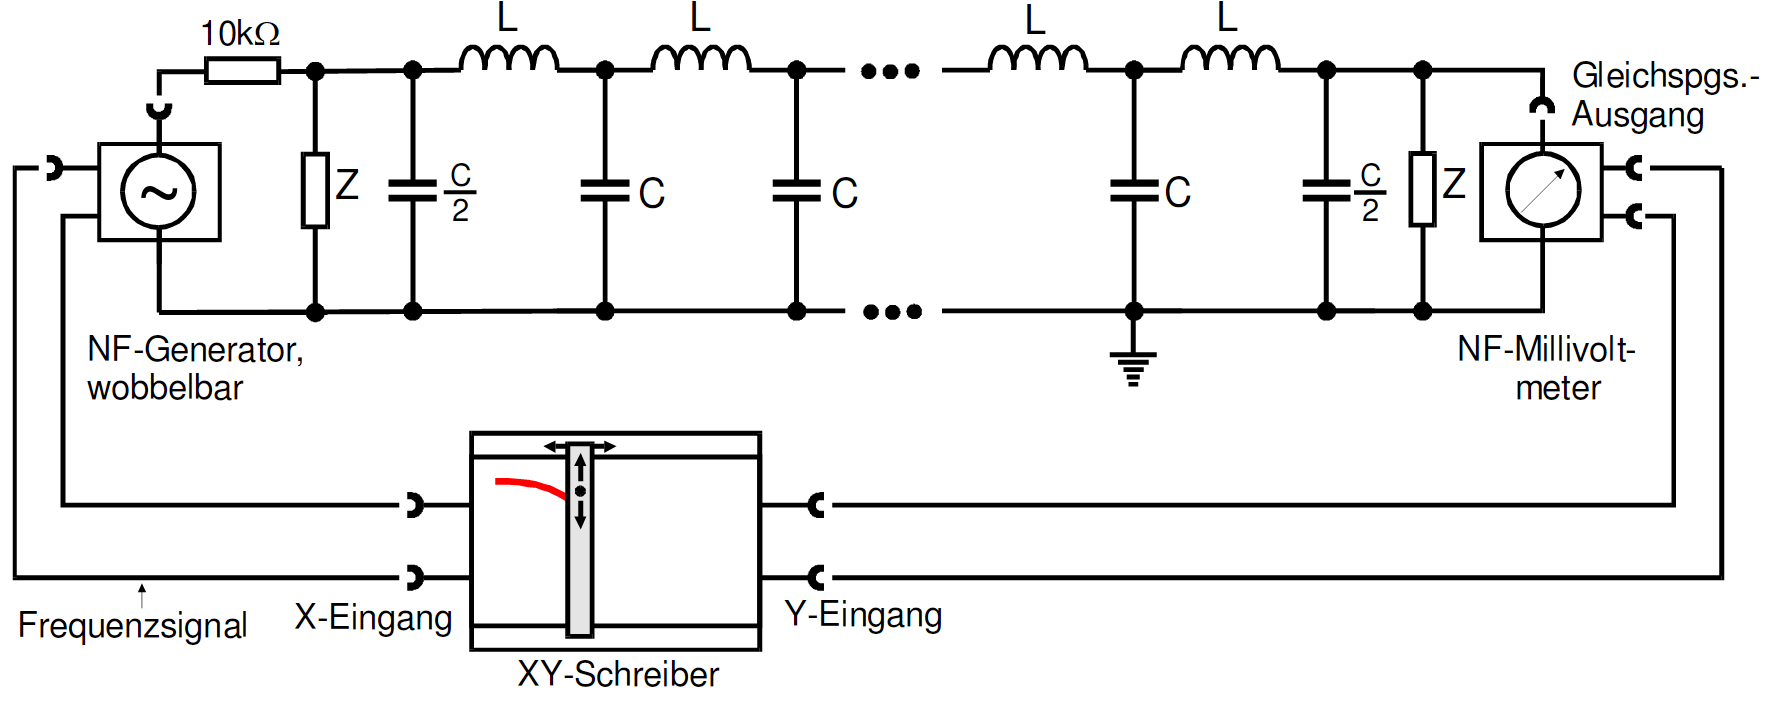
\includegraphics[width=\linewidth-120pt,height=\textheight-120pt,keepaspectratio]{content/Grafiken/Schaltunga.png}
    \caption{Schaltung zum Aufzeichnen der Durchlasskurven [1].}
    \label{fig:Schaltung1}
  \end{figure}

  \item Zunächst werden Durchlasskurven der $LC-$ und $LC_1C_2$-Kette aufgenommen.
   Hierzu wird die jeweilige Kettenschaltung gemäß Abb. 99999 an einen XY-Schreiber
   angeschlossen. Um das Verhalten einer unendlichen Kette zu erzeugen, werden die
   variablen Widerstände an den Enden der Kette auf den nach () berechenbaren
   Wellenwiderstand eingestellt. Am Generator wird eine Sinusspannung gewählt.
    Aufgrund von älteren Geräten wird die Wechselspannungsfrequenz über einen
     Frequenzmesser abgelesen. Auch Anfangs und Endwiderstand werden mithilfe
      eines Ohmmeters justiert. Es ist zu beachten, dass die X-Achse des
       produzierten Graphen $\propto ln(f)$ verläuft.

       \begin{figure}[H]
         \centering
         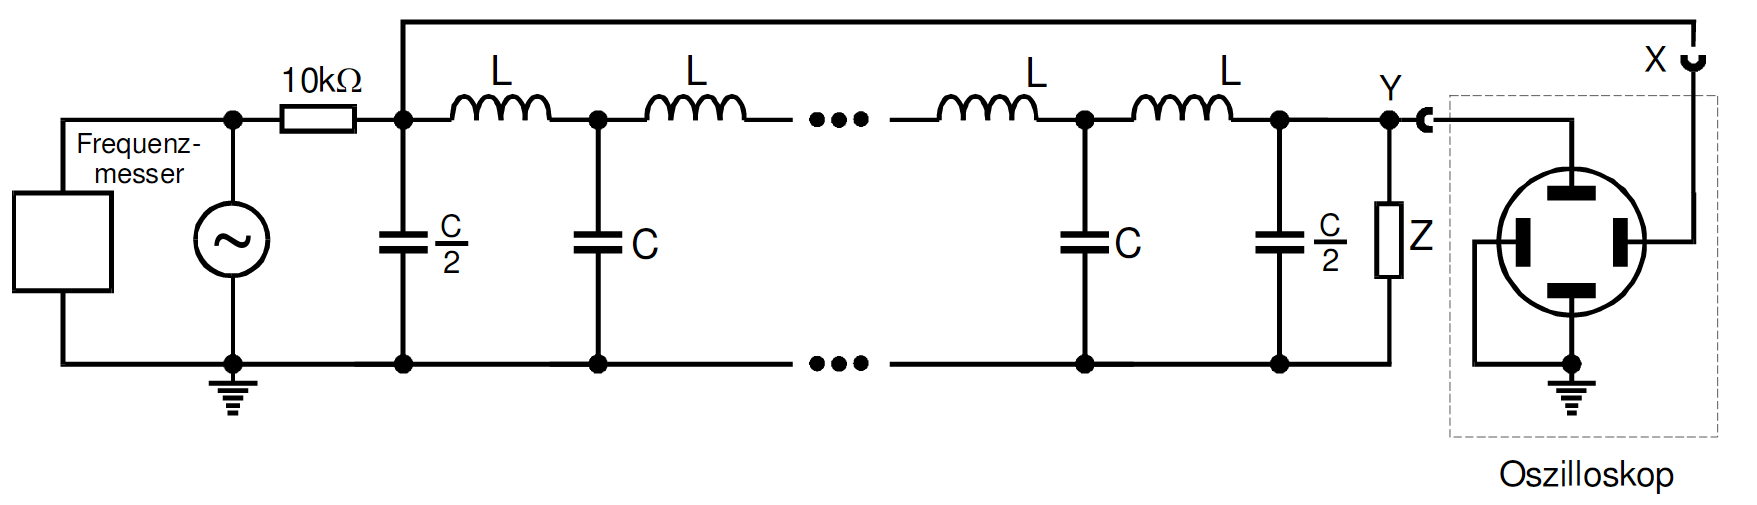
\includegraphics[width=\linewidth-120pt,height=\textheight-120pt,keepaspectratio]{content/Grafiken/Schaltungb.png}
         \caption{Messschaltung zum aufnehmen des Dispersionsverhaltens}
         \label{fig:Schaltung2}
       \end{figure}

\item Als nächstes wird die Dispersionsrelation bestimmt. Hierzu wird die
 Kettenschaltung in eine Schaltung gemäß Abb. 999999 integriert. Das Ossziloskop
  wird auf den XY Modus eingestellt. Anschließend werden alle Frequenzen notiert,
    bei denen die auftretende Lissajous-Figur eine Gerade bildet. Dies ist der
     Fall, wenn die gesamte Phasenänderung auf der Kettenschaltungen ein
      vielfaches von $\pi$ erreicht. Die gesuchte Phasenverschiebung pro Kettenglied
        erreicht man, indem man durch die Anzahl der Kettenglieder teilt.

\item Es wird nun auf eine beiderseits offene LC-Kette gewechselt. Hierzu kann
 die bereits aus Durchführungsteil a) bekannte Schaltung verwendet werden,
  diese mal jedoch ohne Schreiber und Wobbeleinrichtung. Um zwei offene Enden zu
   erreichen werden die Aschlusswiderstände entfernt und der Stromkreis geöffnet.
    Auf der LC-Kette bilden sich nun stehende Wellen. Es
   sollen die Frequenzen notiert werden, bei denen die Spannung am Kettenende
    maximal ist. Hierfür wird ein Millivoltmeter zwischengeschaltet.

\item Anschließend werden bei den ersten beiden Eigenschwingungen auch die
 Spannungen notiert, welche an jedem einzelnen $LC$-Glied anliegen. Hierzu wird
  das ausgehende Kabel nicht mehr am Kettenschaltungsende angebracht, sondern
   am jeweiligen LC-Glied.

   \item Zuletzt wird die voherige Messung nocheinmal durchgeführt. Dieses mal
    wird der Stromkreis jedoch wieder geschlossen, die Abschlusswiderstände werden
     wieder auf den bereits berechneten Wellenwiderstand eingestellt. 


\end{enumerate}
